\begin{tikzpicture}
	\pgfplotsset{/tikz/font={\tiny}}
	\begin{axis}[
			% xlabel={Additional $8\times8$ transforms},
			% ylabel={Y BD-rate (\%)},
			grid=both,
			scale only axis,
			width=0.9\textwidth,
			height=0.6\textheight,
			xtick={0, 1, 2, 4, 8, 16, 32},
			x tick label style={
				rotate=-60, anchor=west,
				/pgf/number format/.cd,
				fixed,
				fixed zerofill,
				precision=0,
			},
			ytick={0,-1,-2,-3,-4,-5,-6},
			y tick label style={
				/pgf/number format/.cd,
				fixed,
				fixed zerofill,
				precision=1,
			},
			% yticklabels={0\%, -1\%, -2\%, -3\%, -4\%, -5\%, -6\%},
			xmin=0, xmax=32,
			ymin=-6, ymax=0,
			% legend entries={sep-$8\times8$,nsep-$8\times8$},
			legend style={nodes=right},
			legend pos= north east,
            xticklabels={DCT, DCT + 1 RDOT, DCT + 2RDOT, DCT + 4 RDOT, DCT + 8 RDOT,
			DCT + 16 RDOT, DCT + 32 RDOT},
		]

		% \pgfplotstableread{figures/prog_transf_8x8.dat}\table
		% \addplot[mark=*,mark size=1.1pt, red, thick, smooth, tension=0.3, dashed]
		% table[x=ntrans,y=sep,col sep=tab] from \table;

		\addplot [mark=*,mark size=1pt, red, thick, dashed] table {
		0	0
		1	-0.9910
		2	-1.4612
		4	-1.8767
		8	-2.2685
		16	-2.6962
		32	-3.1103
		};
		\addlegendentry{separable}

		\addplot [mark=*,mark size=1pt, red, thick] table {
		0	0
		1	-2.8143
		2	-3.6062
		4	-4.2264
		8	-4.8164
		16	-5.3988
		32	-5.9602
		};
		\addlegendentry{non-separable}
	\end{axis}
\end{tikzpicture}
